\documentclass[11pt]{article}
\usepackage{style_template}

\begin{document}

	\hrule
	\begin{center}
        \textbf{MATH103: Complex Analysis}\hfill \textbf{Fall 2023}\newline

		{\Large Compactification: The Riemann Sphere and Projective Space} \\
        David Yang and Yue Zhang
	\end{center}

\hrule

\vspace{1em}

\section{Definitions of Riemann Sphere and Compactification}

\begin{definition}[Riemann Sphere] The \textbf{Riemann Sphere} is a model of the extended complex plane $\mathbb{C}^*$. Intuitively, it is the unit sphere $S^2\subset \mathbb{R}^3$, and its stereographic projection from its north pole $(0,0,1)$ is $\mathbb{C}^*$ (the north pole maps to $\infty$).
\end{definition}
\begin{figure}[ht]
    \centering
    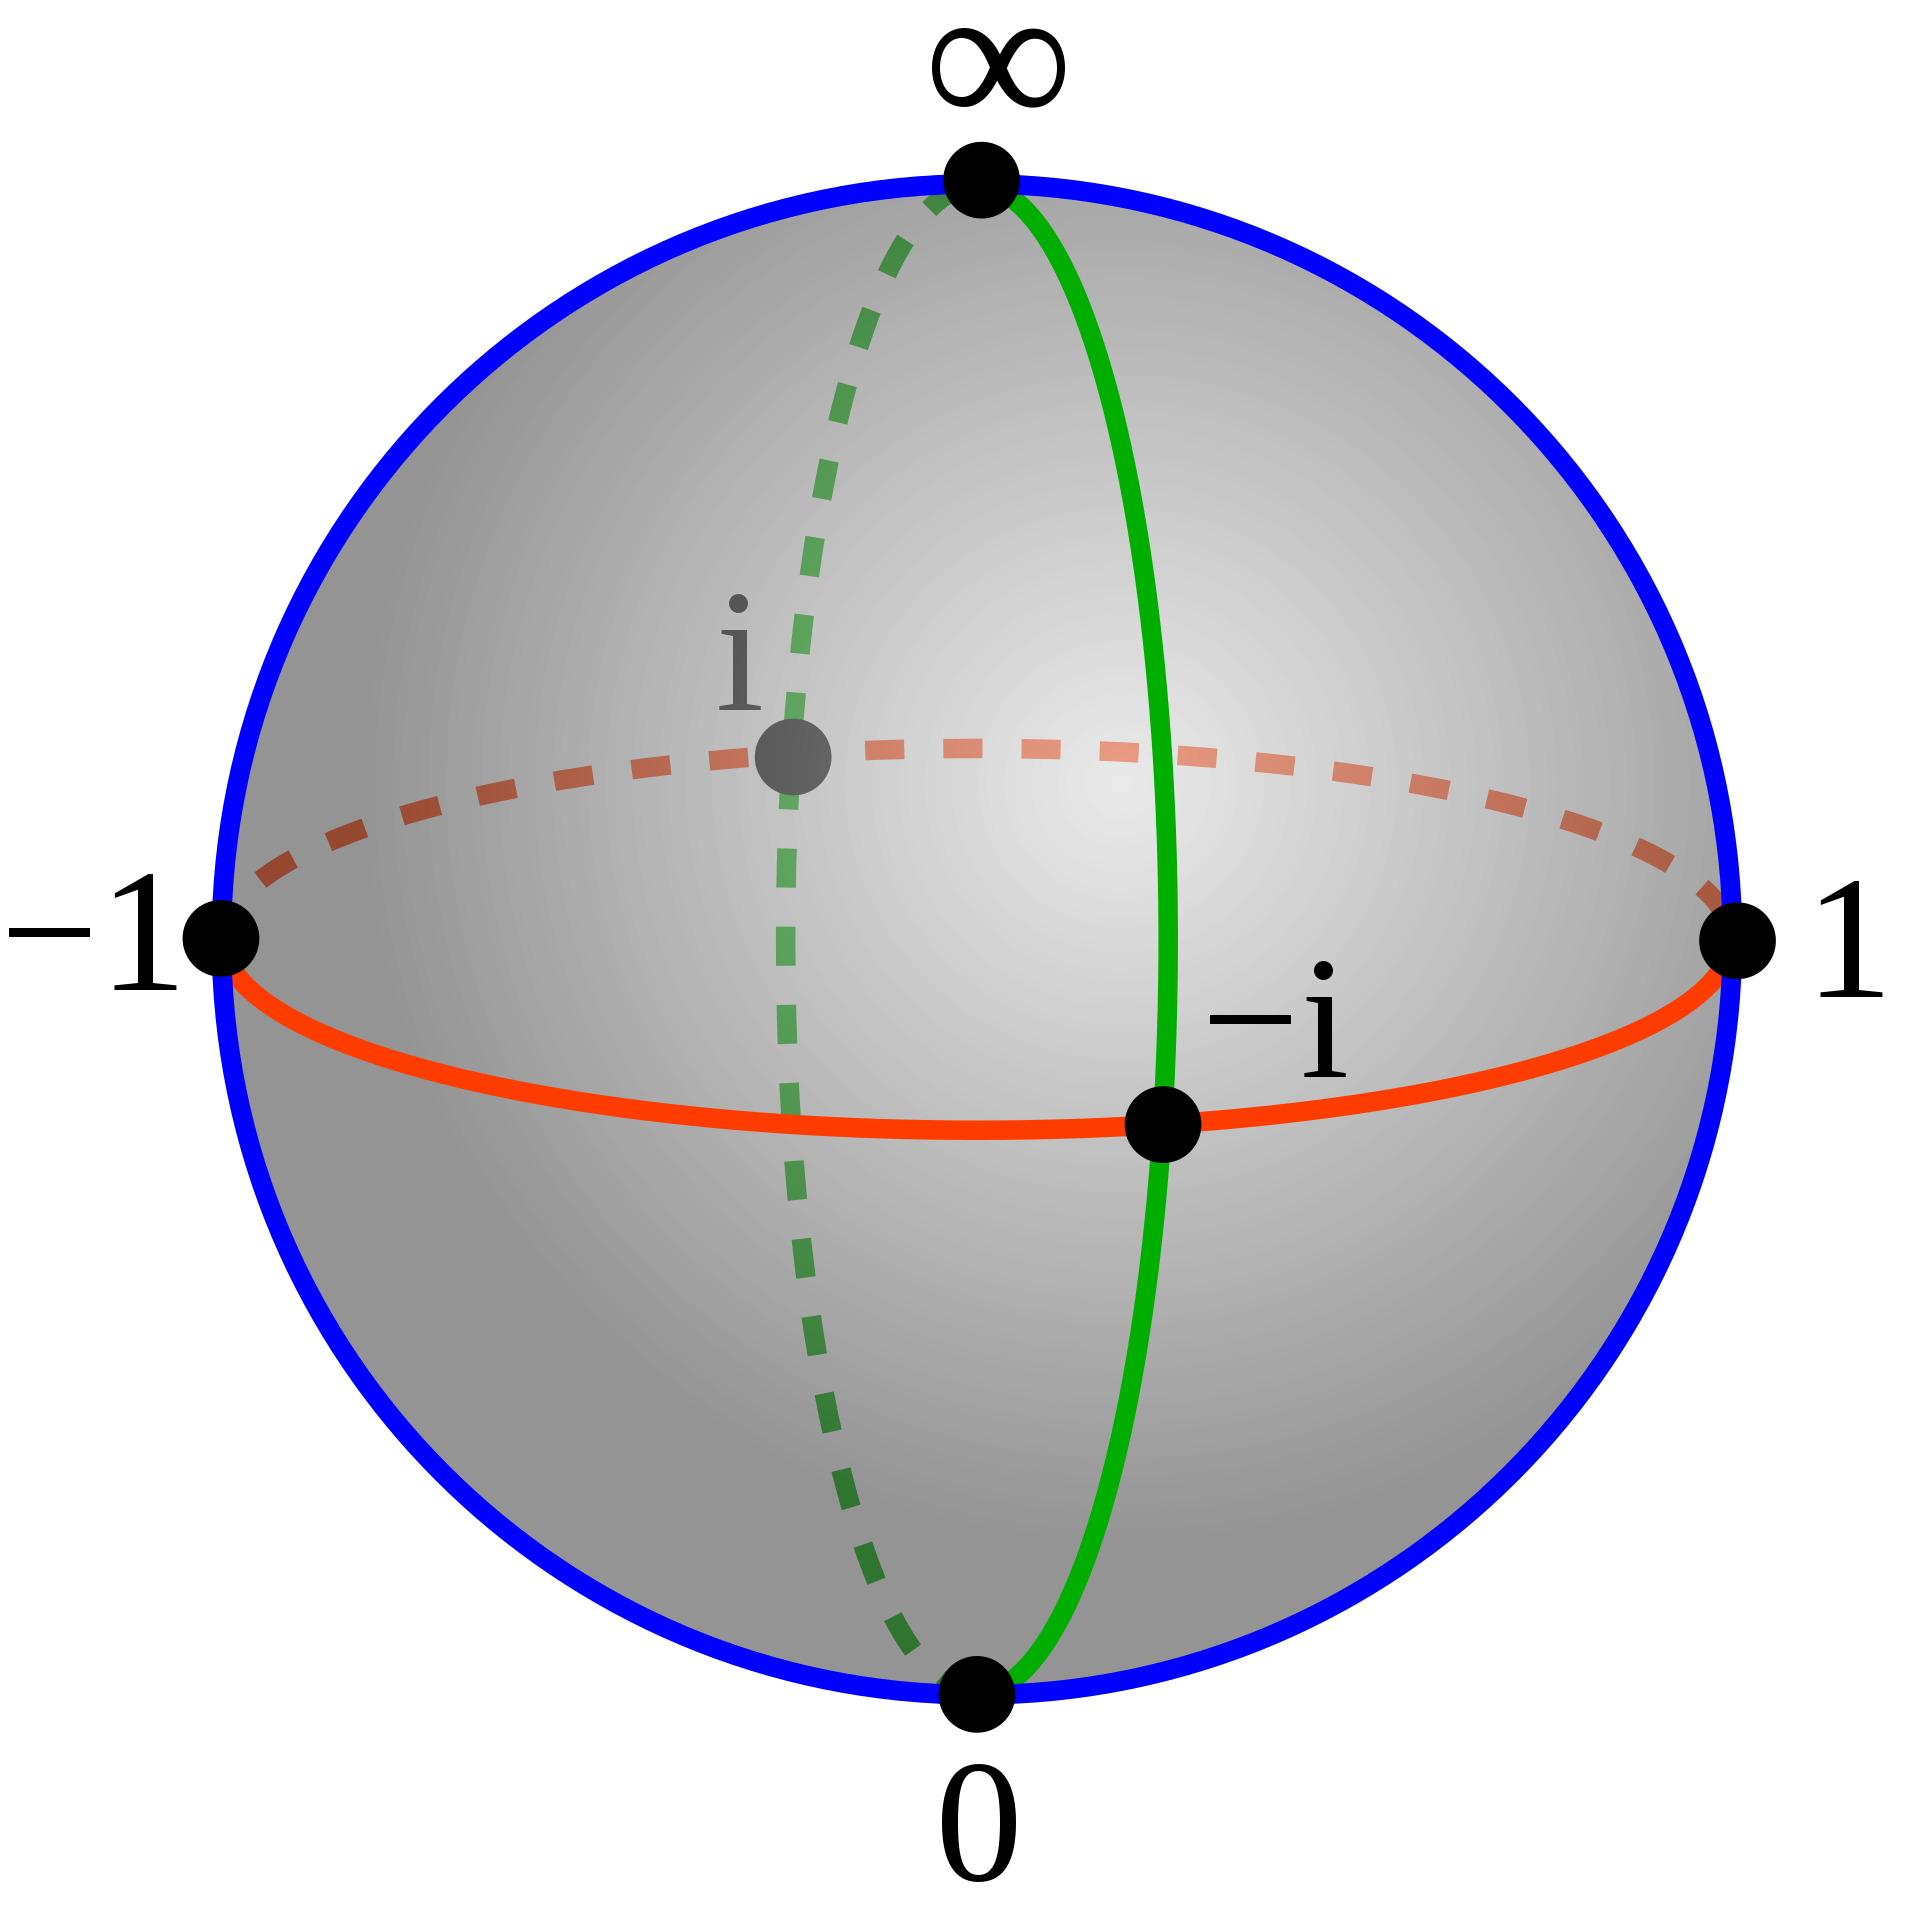
\includegraphics[scale=0.05]{RiemannSphere.png}
    \caption{The Riemann Sphere. Source: Wikipedia}
\end{figure}

We know that $S^2$ is compact. Note that the stereographic projection is conformal from $S^2$ onto $\mathbb{C}^*$, so $\mathbb{C}^*$ is compact. $\mathbb{C}$ is not compact, and we add $\infty$ to it, to make $\mathbb{C}^*=\mathbb{C}\cup \{\infty\}$ compact. We call this process \textbf{compactification}. Note: $\infty$ is not the same in different spaces.  \\

\begin{exercise*} Find a way to compactify $\mathbb{R}^n$. \end{exercise*}

\section{Understanding Projective Space}

Let $\sim$ be the equivalence relation on $\mathbb{C}^{n+1} - \{ 0 \}$ by $x \sim y$ when $\alpha \cdot y$ for some $\alpha \in \C^{\times}$. Equivalently, $x \sim y$ means that $x$ and $y$ lie on the same complex line in $\C^{n+1}.$ \\

\begin{definition}[Complex Projective $n$-space]
    The \textbf{complex projective $n$-space $\CP^{n}$} is the quotient of $\C^{n+1}$ by this equivalence relation:
\[ \CP^n = \frac{(\C^{n+1} - \{0\})}{\sim} \, \, \, \, \approx \, \, \, \, \{ \text{complex lines in } \C^{n+1} \} \]
\end{definition} 
\subsection{An Algebraic Interpretation}

Consider the equation \[ x^N + y^N = 1, \text{which we will call Fermat's Equation 1 (FE1)} \]

for rational $x, y$. This is a version of the well-known Fermat's Last Theorem from Number Theory and will motivate the construction of the projective plane. \\

Suppose we have a solution $(x, y) = (a/c, b/d)$, for $a$, $b$, $c$, $d$ $\in \mathbb{Z}$ with $c$, $d > 0$. \\

\begin{exercise*} Show, by substituting and solving, a solution $(x, y) = (a/c, b/d)$ to \[x^N + y^N = 1\] must satisfy $c = d$. \\

\textit{Hint: Use divisibility rules: if $x \mid y$ and $x \mid z$, then $x \mid (y-z)$ and $x \mid (y+z)$).}
\end{exercise*}

By the above exercise, we know that any solution to FE1 must be of the form $(x, y) = (a/c, b/c)$, which corresponds to the solution $(a, b, c)$ of
\[ X^N + Y^N = Z^N, \text{which we will call Fermat's Equation 2 (FE2).} \]

Conversely, any integer solution $(a, b, c)$ to FE2
with $c \neq 0$ gives a rational solution $(a/c, b/c)$ to FE1; furthermore, more than one solution to FE2 could yield the same solution to FE1. For example, $(ta, tb, tc)$ for $t\neq 0$ is a solution to FE2 that similarly corresponds the solution $(a/c, b/c)$ to FE1. \\

\textit{Conclusion}: This gives some motivation for the equivalence relation discussed previously -- we treat ``multiples'' of the same solution as the same solution.  \\

One minor case to consider is when $N$ is odd. Note that the solutions $(1, -1, 0)$ and $(-1, 1, 0)$ to FE2 have no corresponding rational solutions to FE1. In this instance, we say that these solutions to FE2 actually correspond to solutions of FE1 that lie ``at infinity'' (this is equivalent to treating $1/0 = -1/0 = \infty$). \\

\begin{definition}[Projective Plane, Algebraic]
    For the equivalence relation $\sim$ where $[a, b, c] \sim [a', b', c']$ if $a = ta', b=tb', c=tc'$ for some nonzero $t$, the projective plane $\mathbb{P}^2$ is
\[ \mathbb{P}^2 = \frac{\{[a, b, c] : a, b, c \text{ are not all zero} \}}{\sim}.\]
\end{definition}

The numbers $a, b, c$ give the \textbf{homogeneous coordinates} for the point $[a, b, c]$ in projective space. Note that our notion of a projective plane can be extended to any \textbf{projective $n$-space} which has a similar definition, as the set of equivalence classes of homogeneous $n+1$ tuples. \\

\subsection{A Geometric Interpretation}

\begin{definition}[Projective Line, Geometric]
A \textbf{projective line} in $\mathbb{P}^2$ is a set of points $[a, b, c] \in \mathbb{P}^2$ whose coordinates satisfy \[\alpha X + \beta Y + \gamma Z = 0\] for some constants $\alpha, \beta, \gamma$ not all equal to $0$.
\end{definition} 

Just as we do in the Euclidean plane, we want two non-parallel lines to intersect at a unique point in the projective plane. However, two parallel lines should similarly intersect; as we've seen before, it might make sense to have these lines intersect at the point at infinity, which they do. But is one point of infinity enough? It turns out that it is not. 
\begin{center}
    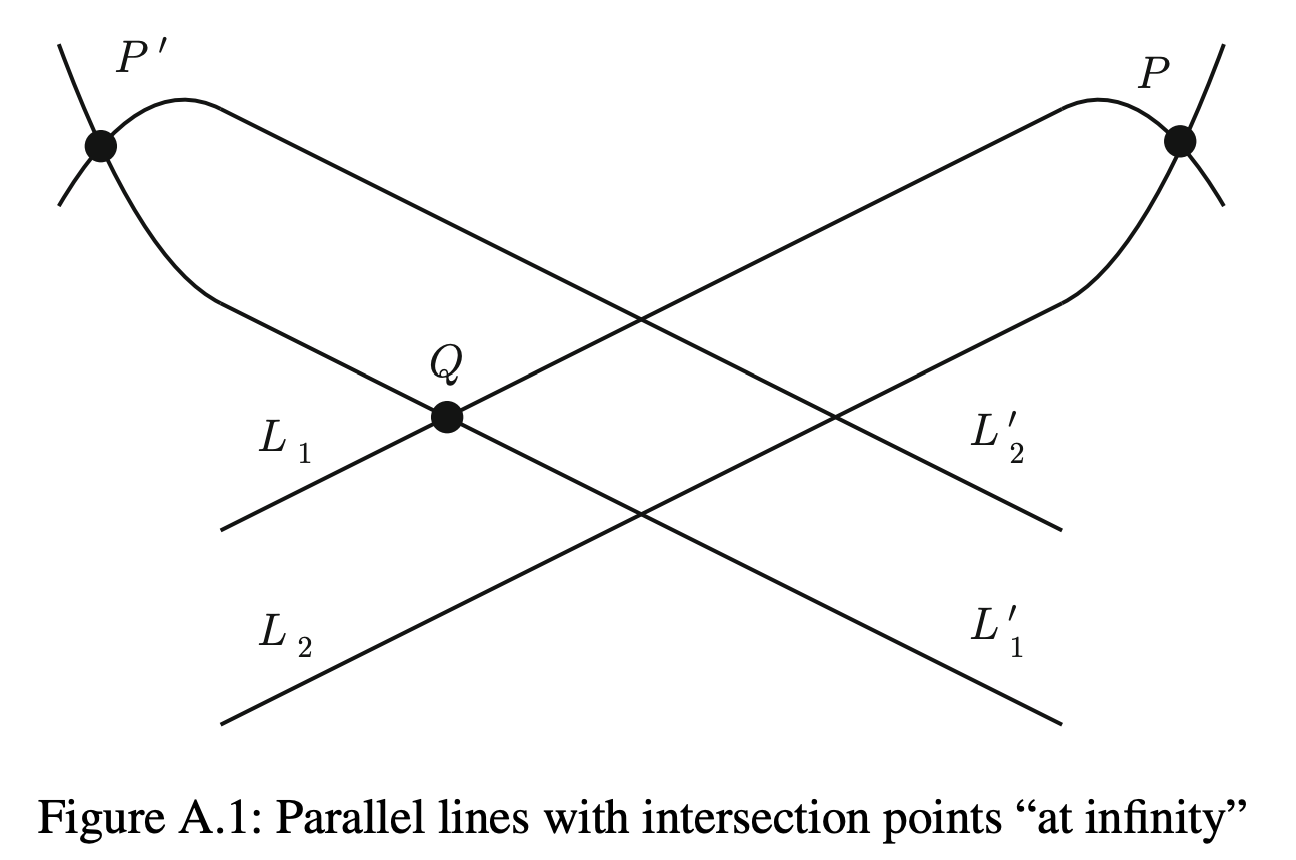
\includegraphics[scale=0.5]{ProjectiveLineIntersection.png}
\end{center}

In the above construction, lines $L_1, L_2$ and $L'_1$ and $L'_2$ are parallel, and so they intersect at points at infinity $P$ and $P'$. Consider lines $L_1$ and $L'_1$ which are not parallel to each other. They intersect at a point $Q$, and if $P = P'$, also at the point at infinity. \\

To maintain the property that two non-parallel lines intersect at just one point, we need the two points at infinity $P$ and $P'$ to be distinct. Thus, a pair of parallel lines intersects at a point at infinity that is determined by the direction of that line (equivalently, there is an extra point at infinity for each direction of the projective plane). \\

\begin{definition}[Affine and Projective Plane, Geometric] The \textbf{affine plane} (the usual Euclidean plane) is
\[ \mathbb{A}^2 = \{ (x, y): x \text{ and } y \text{ are numbers} \}\]

The \textbf{projective plane} can be defined as
\[\mathbb{P}^2 = \mathbb{A}^2 \cup \{\text{the set of directions in } \mathbb{A}^2 \}.\]
\end{definition}

The points associated to directions can be understood as \textbf{points at infinity}, with the notion that parallel lines have the same direction. \\

\textit{Note}: A given direction in $\mathbb{A}^2$ can be understood by a parallel line to that direction passing through the origin. Since the equation of this line can be represented as $Ay = Bx$ with $A, B$ not both zero, we can consider the pair $(A, B)$ as a representative for this line. Furthermore, since $(A, B)$ and $(A', B')$ are the same line if and only if $A = tA'$ and $B = tB'$, we can naturally describe the set of directions $\mathbb{A}^2$ as points $[A, B]$ of the projective line $\mathbb{P}^1.$ So another natural definition for the projective plane is 
\[\mathbb{P}^2 = \mathbb{A}^2 \cup \mathbb{P}^1.\]

These give equivalent algebraic and geometric definitions of the projective plane, summarized in the following table:
\begin{center}
    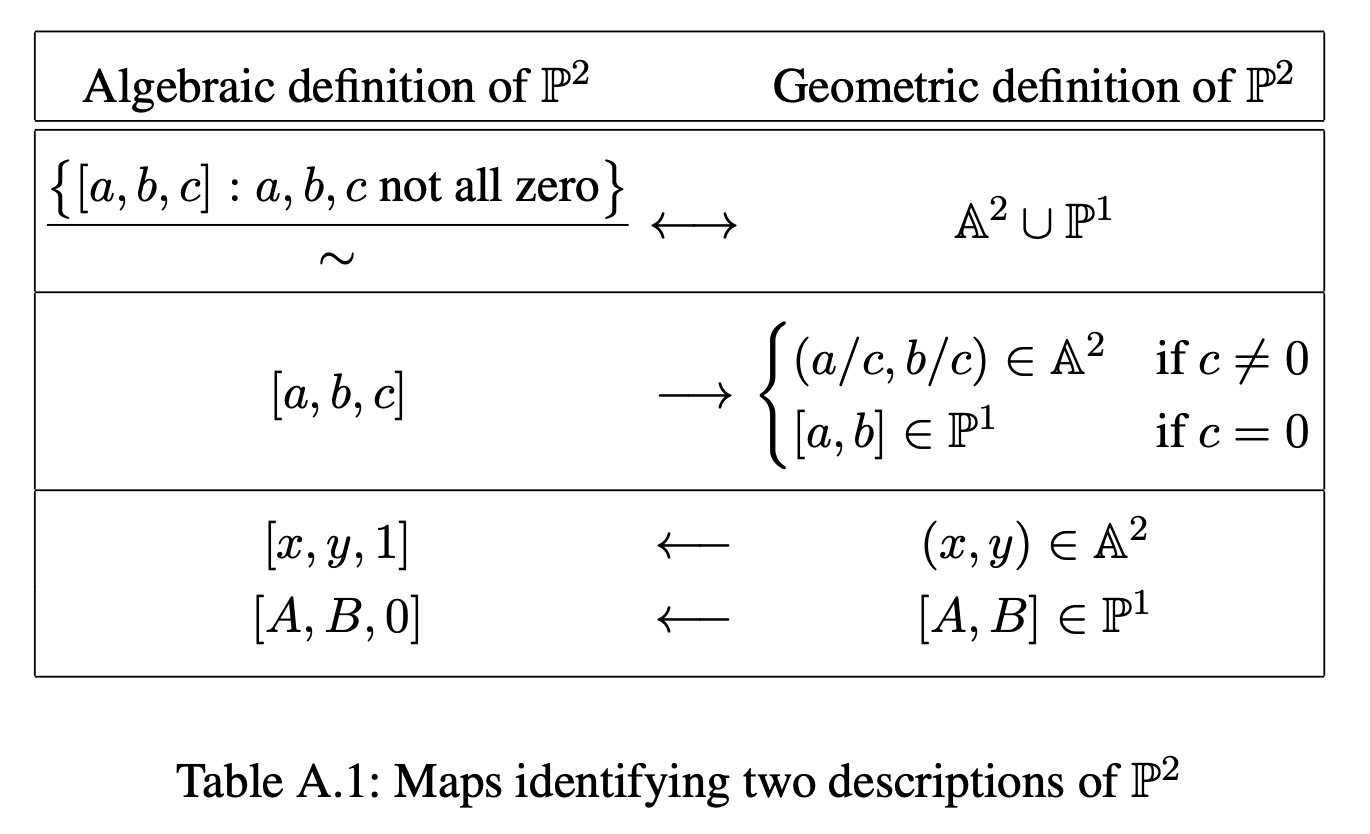
\includegraphics[scale=0.5]{ProjectivePlaneDefinitions.png}
\end{center}

\section{Intersection of Curves in the Projective Plane}

\begin{definition} An \textbf{algebraic curve} in the affine plane $\mathbb{A}^2$ is defined to be the set of solutions
to a polynomial equation in two variables: \[ f(x, y) = 0.\]

\textit{Note}: Since points in the projective plane are represented by a homogeneous triple, curves must be defined by polynomials in three variables. \\

A polynomial $F(X, Y, Z)$ is a \textbf{homogeneous polynomial of degree $d$} if it satisfies the identity
\[ F(tX, tY, tZ) = t^d F(X, Y, Z).\]

A \textbf{projective curve} $C$ in the projective plane is the set of solutions to a homogeneous polynomial equation
\[ F(X, Y, Z) = 0.\]
\end{definition}

We conclude with a powerful theorem in algebraic geometry, Bezout's Theorem. \\

\begin{theorem}[Bezout's Theorem] Suppose that $C_1$ and $C_2$ are two projective curves of degrees $d_1$ and $d_2$ with no ``common components.''\footnote{the definition of this concept requires further machinery: see \cite{silverman} if interested.} \\

Then $C_1$ and $C_2$ intersect at $d_1d_2$ points, counted with their multiplicity, and including points at infinity and points with complex coordinates.
\end{theorem}

\begin{exercise*}
How many intersections do two projective curves of degree $3$ and $5$ have, if they have no common components?   
\end{exercise*}


\begin{thebibliography}{9}
\bibitem{silverman}
Joseph H. Silverman, John T. Tate (2015). \emph{Rational Points on Elliptic Curves}, Springer Nature.

\bibitem{garrett}
Paul Garrett (2014). \emph{Compactification: Riemann sphere, projective space}.
\end{thebibliography}

\newpage

\section{Solutions to Exercises}

\begin{solution*} In the general case of $\mathbb{R}^n$, the stereographic projection comformally maps from $S^n$ to $\mathbb{R}^n\cup \{\infty\}$, in which $\infty$ is defined to be the image of the north pole $(0,0,...,1)$, and the inclusion of $\infty$ is a compactification for $\mathbb{R}^n$.
\end{solution*}

\begin{solution*}
Substitute $x = a/c$ and $y = b/d$ to FE1, and multiply both sides by $c^N d^N$ to clear the fractions of their denominators. This gives
\[ a^N d^N + b^N c^N = c^N d^N.\]

Since $c^N \mid b^N c^N$ and $c^N \mid c^N d^N$, we must have that $c^N \mid a^N d^N.$ Since $a$, $c$ are relatively prime by construction, this tells us that $c \mid d.$ \\

By a similar line of logic, since $d^N \mid a^N d^N$ and $d^N \mid c^N d^N$, we must have that $d^N \mid b^N c^N.$ Again, since $b$, $d$ are relatively prime by construction, we conclude that $d \mid c.$ \\

Since $c \mid d$ and $d \mid c$, $c = d$, as desired. Thus, all solutions to FE1 are of the form \[(x, y) = \left( \frac{a}{c}, \frac{b}{c} \right).\]\end{solution*}

\begin{solution*}
By Bezout's Theorem, projective curves of degrees $3$ and $5$ with no common components intersect at $3 \cdot 5 = 15$ points.
\end{solution*}

\end{document}
